\chapter{Living in the Future}

``Live in the present'' is one of those phrases that sounds wise because it is comforting. It reminds people not to waste life in regret, fantasy, or anxiety. In that limited sense, it has value. But as a principle for building wealth freedom, it is dangerously incomplete.

If a person only lives in the present, the present becomes a cage. There is no direction, no compounding, no preparation, and no reason to endure temporary discomfort. The person reacts to what appears today, consumes what is available today, and protects the feeling of being safe today. The future remains a vague space that will arrive by itself.

That is not freedom. That is being trapped in an eternal now.

\begin{center}
\begin{adjustbox}{max width=\linewidth}
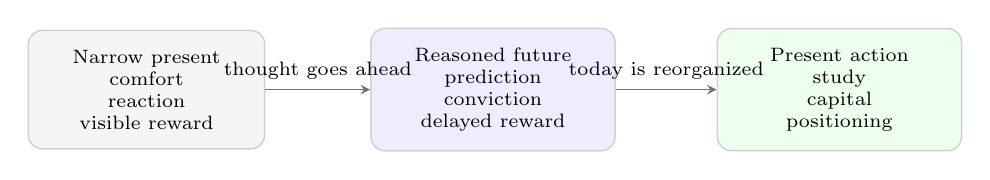
\begin{tikzpicture}[font=\scriptsize, line width=0.55pt, >=stealth]
  \node[draw=black!18, fill=gray!8, rounded corners=5pt, align=center, inner sep=7pt, minimum width=3.0cm] (now) at (0,0) {Narrow present\\comfort\\reaction\\visible reward};
  \node[draw=black!18, fill=blue!7, rounded corners=5pt, align=center, inner sep=7pt, minimum width=3.1cm] (future) at (4.4,0) {Reasoned future\\prediction\\conviction\\delayed reward};
  \node[draw=black!18, fill=green!7, rounded corners=5pt, align=center, inner sep=7pt, minimum width=3.1cm] (action) at (8.8,0) {Present action\\study\\capital\\positioning};
  \draw[->, draw=black!55] (now) -- node[above]{thought goes ahead} (future);
  \draw[->, draw=black!55] (future) -- node[above]{today is reorganized} (action);
\end{tikzpicture}
\end{adjustbox}
\end{center}

A better foundation for life is this:

\begin{quote}
One must learn to live, at least partly, in the future.
\end{quote}

This sounds abstract, but the practice is simple.

\begin{enumerate}
\item You make a prediction about the future.
\item The prediction needs time before it can be verified.
\item You develop firm conviction that the prediction is probably right.
\item You begin to act, choose, and think according to that future result.
\item Time passes, and the future eventually arrives.
\item If the prediction proves correct, then during the waiting period part of your life was already being lived in that future.
\end{enumerate}

This is not magic. It is disciplined imagination joined to action. The body can only live in the present, but thought does not have to stay there. Thought can project, compare, prepare, and allocate today's resources according to tomorrow's likely reality.

\section*{The Width of the Present}

The present is not the same size for everyone.

For a person who never thinks seriously about the future, the present is narrow. It contains only immediate feelings, visible incentives, current problems, and current opinions. The future may exist as a word, but it has no practical weight.

For a person who has made a few serious predictions, the present becomes wider. Tomorrow begins to influence today. Choices are no longer made only by asking, ``What do I want now?'' They are made by asking, ``What will this choice look like after time has done its work?''

\begin{center}
\begin{adjustbox}{max width=\linewidth}
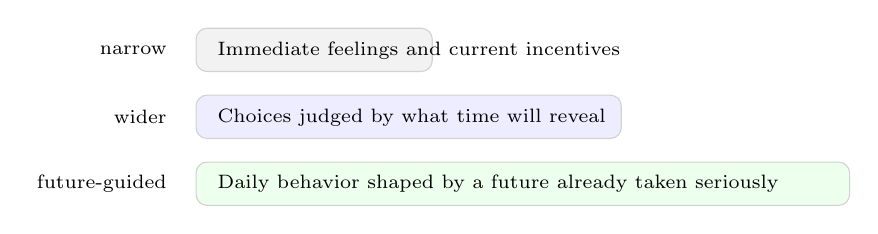
\begin{tikzpicture}[font=\scriptsize]
  \draw[fill=gray!10, draw=black!18, rounded corners=4pt] (0,0) rectangle (3.0,0.55);
  \node[anchor=west] at (0.15,0.27) {Immediate feelings and current incentives};
  \draw[fill=blue!7, draw=black!18, rounded corners=4pt] (0,-0.85) rectangle (5.4,-0.30);
  \node[anchor=west] at (0.15,-0.58) {Choices judged by what time will reveal};
  \draw[fill=green!7, draw=black!18, rounded corners=4pt] (0,-1.70) rectangle (8.3,-1.15);
  \node[anchor=west] at (0.15,-1.43) {Daily behavior shaped by a future already taken seriously};
  \node[anchor=east, align=right] at (-0.25,0.27) {narrow};
  \node[anchor=east, align=right] at (-0.25,-0.58) {wider};
  \node[anchor=east, align=right] at (-0.25,-1.43) {future-guided};
\end{tikzpicture}
\end{adjustbox}
\end{center}

For a person who has thought deeply, the overlap becomes larger still. The future is not a distant idea. It presses into daily behavior. Such a person can sacrifice entertainment, study an unfashionable skill, endure loneliness, pay for better knowledge, leave a comfortable track, or build patiently while others ask why the reward has not appeared yet.

\begin{center}
\begin{adjustbox}{max width=\linewidth}
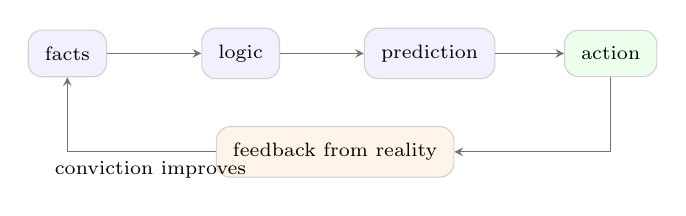
\begin{tikzpicture}[font=\scriptsize, >=stealth]
  \node[draw=black!18, fill=blue!6, rounded corners=5pt, align=center, inner sep=6pt] (facts) at (0,0) {facts};
  \node[draw=black!18, fill=blue!6, rounded corners=5pt, align=center, inner sep=6pt] (logic) at (2.2,0) {logic};
  \node[draw=black!18, fill=blue!6, rounded corners=5pt, align=center, inner sep=6pt] (prediction) at (4.6,0) {prediction};
  \node[draw=black!18, fill=green!7, rounded corners=5pt, align=center, inner sep=6pt] (action) at (6.9,0) {action};
  \node[draw=black!18, fill=orange!9, rounded corners=5pt, align=center, inner sep=6pt] (feedback) at (3.4,-1.25) {feedback from reality};
  \draw[->, draw=black!55] (facts) -- (logic);
  \draw[->, draw=black!55] (logic) -- (prediction);
  \draw[->, draw=black!55] (prediction) -- (action);
  \draw[->, draw=black!55] (action) |- (feedback);
  \draw[->, draw=black!55] (feedback) -| node[pos=0.22, below]{conviction improves} (facts);
\end{tikzpicture}
\end{adjustbox}
\end{center}

Most people do not lack slogans about the future. They lack conviction. They have heard that knowledge matters, that time compounds, that attention is precious, that capital changes the structure of life. Yet they have not thought long enough to believe these statements with enough force to act.

There is a large difference between knowing a sentence and living by it.

\section*{Prediction Requires the Loss of Perfect Security}

The previous chapter argued that the demand for 100\% security prevents growth. This chapter shows one important reason: prediction always contains uncertainty.

A person who insists on certainty before acting cannot live in the future. The future is never available with complete proof. Data can be incomplete. Logic can be wrong. Timing can be off. Even a correct direction may take longer than expected.

So the practice is not to eliminate uncertainty. The practice is to reason as well as possible, act in advance, and then let reality test the reasoning.

This is why living in the future is rare. Many people want the reward of a correct prediction, but they do not want the discomfort of acting before the crowd agrees. They want to be early only after everyone has confirmed that early was right. That is impossible.

If you wait until the result is obvious, you are no longer living in the future. You are merely obeying the present.

\section*{A Plain Prediction: Knowledge Beats Force}

Consider a simple prediction:

\begin{itemize}
\item Over the long term, mental output will have much higher productivity than physical output.
\item Physical strength has an obvious ceiling; intellectual growth has a much less visible ceiling.
\item Physical strength declines relatively early; intellectual capacity can continue improving for much longer.
\item The extreme profits once gained through violence will keep shrinking, because knowledge will become a more powerful source of wealth.
\end{itemize}

Today, this may sound obvious. But obviousness after the fact is cheap. The useful question is whether a person believed it early enough, deeply enough, and practically enough to live differently.

In the 1980s, phrases such as ``knowledge is power'' and ``science and technology are productive forces'' were already common. Many people heard them. Many repeated them. Far fewer built their lives around them.

The important move was not hearing the sentence. The important move was thinking it through until it became a guiding belief. If knowledge will become more productive than physical force, then the rational life strategy is clear: learn, read, think, write, compute, teach, invest in skill, and stay close to fields where knowledge can multiply.

Years later, books such as \emph{Freakonomics} described how street gangs could involve great danger while producing surprisingly poor economic results for many participants. At roughly the same time, young programmers could build games or software and earn far more without the same physical danger. The old prediction did not require genius. It required taking a plain truth seriously before its consequences became visible to everyone.

That is often enough.

\section*{The Difference Between Thought and Deep Thought}

Almost everyone has heard that knowledge is valuable. Why did that knowledge not change everyone's life?

Because most people only let the idea pass through the mind. They did not examine it, challenge it, connect it to action, and return to it again and again. Without that process, no conviction forms.

\begin{quote}
Without deep thought, a person cannot firmly believe their own prediction.
\end{quote}

Mere belief is weak. It disappears when friends laugh, when results are delayed, when the market turns, when parents object, when the crowd moves elsewhere, or when comfort calls. Firm conviction is different. It is not blind confidence. It is confidence produced by repeated reasoning, evidence, questioning, and practice.

This is why many people know the right thing and still do not benefit from it. They know that attention is precious, but spend it casually. They know that time cannot be sold forever, but sell it without building anything. They know that knowledge compounds, but consume information instead of forming ability. They know that paying can be cheaper than wasting time, but still choose free material at the cost of years.

The problem is not always ignorance. Often it is insufficient conviction.

\section*{Another Prediction: Paid Communities}

A more concrete example comes from the rise of online communities.

Around 2014 and 2015, one could reason toward several conclusions:

\begin{enumerate}
\item Communities that seemed to have faded would return.
\item The new generation of communities would outnumber the older generation.
\item Paid communities would gradually become stronger than free ones.
\item Sharing centered on transactions would become more important than sharing centered only on information.
\item The real barriers for a community would likely be payment and accumulated content.
\end{enumerate}

None of these conclusions was guaranteed. They were predictions. But once they were formed, the next question was practical: what should be done now if this future is likely?

The answer was to start building. Open a public account. Accumulate readers. Design paid groups. Help others build their own communities. Develop tools and infrastructure. Use one community as a model room that can be copied and adapted.

Many people will ignore such a prediction before it becomes obvious. That is normal. In fact, a prediction that already receives universal applause may no longer contain much opportunity. The opportunity exists precisely because the future has not yet become common sense.

But this also means the prediction may be wrong. Paid communities might not have become normal. Free communities might have remained dominant. The timing might have failed. The structure might have evolved differently.

That possibility does not invalidate the method. It only reminds us of the rule:

\begin{quote}
Do not expect to be right on the first try.
\end{quote}

Prediction is a practice. Each attempt reveals weaknesses in observation, missing data, lazy assumptions, and loose logic. Failure is not useless if it improves the next prediction.

\section*{Respect Facts, Trust Logic}

There is no universal formula for prediction. Anyone selling a formula that always works is probably selling comfort, not judgment.

Still, two principles are indispensable:

\begin{quote}
Respect facts. Trust logic.
\end{quote}

Respecting facts means seeing what is there, not what would make you feel safe. It means noticing incentives, prices, behavior, technology, regulation, human desire, and actual constraints. It means reading widely enough to avoid being trapped in your own tiny environment.

Trusting logic means connecting facts without forcing them. It means asking what must follow if the premises are true. It means distinguishing trend from noise, cause from coincidence, and preference from evidence.

Both are difficult because the mind is full of bias. We protect old beliefs. We imitate nearby people. We overvalue vivid stories. We confuse familiarity with truth. We avoid conclusions that demand action. Prediction improves only when these habits are repeatedly exposed.

A useful daily exercise is simple: spend thirty minutes predicting what may happen tomorrow or next week. Then ask which of your predictions are things most people around you have not noticed. At first, the answer may be disappointing. That is fine. The weakness exists because the habit has not been trained.

Another exercise is to look at your circle and ask: who has the strongest predictive ability? Why have you not built a deeper relationship with that person? Why have you not had more serious conversations with them? A person's future is strongly affected by the quality of the minds they regularly engage.

\section*{Acting Before the Proof}

Living in the future requires action. A prediction that does not change behavior is only entertainment.

If you believe knowledge will become more valuable, then your calendar must show study, practice, writing, building, teaching, or technical creation. If you believe attention is your most important asset, then your phone, desk, subscriptions, and social habits must reflect that belief. If you believe capital matters, then your spending and saving must begin to form capital. If you believe a field will grow, then you must acquire the skills, relationships, and position that will matter when it does.

This is also the bridge to investing.

\begin{quote}
Investment is the exchange of present resources for future resources.
\end{quote}

That sentence alone explains why people who live in the future tend to accumulate more wealth than people who only live in the present. Investment requires the future to be real enough in your mind that you are willing to give up something now. Without that, every investment feels like loss, every delay feels unbearable, and every fluctuation feels like danger.

The investor, the builder, the writer, the teacher, the founder, and the serious learner all share one structure: they place present attention, time, money, or comfort into a future they believe can become real.

\section*{Seven Years as a Life}

When old knowledge becomes a chain, one helpful mental model is to treat seven years as a lifetime.

This life has its own achievements, habits, identity, and pride. The next life can be different. A person does not have to despise past accumulation in order to move forward. But neither should they let past accumulation define the boundary of all future action.

Industries change. Tools change. Distribution changes. What once looked secure may become weak. What once looked strange may become normal. Even groups built on violence are eventually dragged by the age; they do not get to freeze history in place. If they must adapt, so must everyone else.

The point is not to abandon every field whenever a new fashion appears. Accumulation matters. Deep skill matters. Reputation matters. But one's mind should not be imprisoned by the fact that effort has already been spent.

A person on the road to wealth freedom must be able to say: this chapter of life was real, but it is not the whole book.

\section*{A Practice for This Chapter}

Write down the most important correct prediction you have ever made. Why was it important? Did you act on it early enough?

Then write down the largest prediction you made but failed to benefit from. Why did you not benefit? Did you lack conviction? Capital? Skill? Courage? Time? Partners? Did you fail to convert thought into action?

Finally, choose one plain but deep principle that you already claim to believe. Examples include:

\begin{itemize}
\item Knowledge compounds.
\item Attention is more valuable than money.
\item Paying for quality can be cheaper than wasting time.
\item Selling time forever cannot lead to wealth freedom.
\item Investment exchanges present resources for future resources.
\end{itemize}

Do not merely agree with it. Think through its consequences. Ask what would change this week if you truly believed it. Then make one small change that proves the belief has entered your life.

\section*{The Foundation}

Living in the future is not fortune-telling. It is the discipline of allowing a reasoned future to shape present behavior.

You will be wrong many times. You will act early and look strange. You will receive less encouragement than you hope for. Treat encouragement as a bonus, not as fuel. The fuel must be facts, logic, repeated thought, and action.

If you manage to live in the future even once, the reward can be enormous. More importantly, after one clear experience, the mode becomes easier to repeat. You begin to understand that the present is not merely a place to consume. It is the only place where the future can be purchased.

The body remains here. The mind can go ahead. Wealth freedom begins when enough of the mind refuses to stay trapped in the eternal present.
